\documentclass[runningheads]{llncs}
\usepackage[utf8]{inputenc}
\usepackage{graphicx}
\usepackage{amsmath}
\usepackage{amsfonts}
\usepackage{amssymb}
\usepackage{diagbox}
\usepackage[caption = false]{subfig}
\usepackage[english,main=spanish]{babel}
% If possible, figure files should be included in EPS format.
%
% If you use the hyperref package, please uncomment the following line
% to display URLs in blue roman font according to Springer's eBook style:
% \renewcommand\UrlFont{\color{blue}\rmfamily}


\begin{document}
%
\title{Crossligual visual-based Author Profiling}

%\titlerunning{Abbreviated paper title}
% If the paper title is too long for the running head, you can set
% an abbreviated paper title here

\author{First Author\inst{1}\orcidID{0000-1111-2222-3333} \and
Second Author\inst{2,3}\orcidID{1111-2222-3333-4444} \and
Third Author\inst{3}\orcidID{2222--3333-4444-5555}}
%
\authorrunning{F. Author et al.}
% First names are abbreviated in the running head.
% If there are more than two authors, 'et al.' is used.
%
\institute{Princeton University, Princeton NJ 08544, USA \and
Springer Heidelberg, Tiergartenstr. 17, 69121 Heidelberg, Germany
\email{lncs@springer.com}\\
\url{http://www.springer.com/gp/computer-science/lncs} \and
ABC Institute, Rupert-Karls-University Heidelberg, Heidelberg, Germany\\
\email{\{abc,lncs\}@uni-heidelberg.de}}

\maketitle

\begin{abstract}
The abstract should briefly summarize the contents of the paper in
150--250 words.

\keywords{First keyword  \and Second keyword \and Another keyword.}
\end{abstract}

\section{Introducción}

El contenido compartido en redes sociales incluye información 
en distintas modalidades como texto, imágenes, audio y video.
Todos estos datos pueden utilizarse para extraer información
valiosa de los usuarios. 
La tarea de perfilado de autores (AP por sus siglas en inglés), a través
del análisis de contenido compartido, busca determinar características demográficas 
específicas como género, edad, personalidad, legua nativa u orientación 
política \cite{rangel_rosso_montes-y-gomez_potthast_stein}. La identificación de tales
aspectos puede aplicarse en una gran variedad de campos. Por ejemplo, la detección del
género es útil en márketing y publicidad, donde las empresas pueden estar interesadas
en si le gustará o no un producto a un grupo demográfico \cite{miller_dickinson_hu_2012}.
También, dentro de la criminalística, es de interés detectar cuando alguien falsifica su género en internet \cite{cheng_chandramouli_subbalakshmi_2011}. 


Existen varias conferencias cuya meta 
es promover la investigación en áreas de recuperación
de información. Entre ellas están la Text REtrieval Conference (TREC) y la 
iniciativa CLEF (Conference and Labs of the Evaluation Forum, anteriormente 
conocida como Cross-Language Evaluation Forum). Dentro de esta última, se 
encuentra el PAN, una serie de eventos científicos y tareas sobre textos 
forenses y estilometría de textos digitales.
%  \cite{pan}. 

El objetivo de la tarea
de perfilado de autores del PAN 2018 fue abordar la identificación de género
desde una perspectiva multimodal donde además de texto se
incluyeron imágenes \cite{rangel_rosso_montes-y-gomez_potthast_stein}.
Para cumplir el propósito de la tarea, se brindó un conjunto de datos
obtenido de Twitter, el cual comprende tres idiomas: árabe, inglés y español.
La tarea permitía la clasificación para un subconjunto de idiomas; usando sólo texto, imágenes o haciendo una fusión de las dos fuentes de información.

A partir de los resultados obtenidos usando sólo imágenes 
 \cite{rangel_rosso_montes-y-gomez_potthast_stein}, se pudo observar que es posible 
utilizar información de éstas para el perfilado de usuarios.
La hipótesis de este trabajo es que las imágenes de una colección para un
idioma  pueden ser útiles para identificar el perfil en otro idioma. 
Lo anterior es útil cuando no se cuenta con la cantidad suficiente de datos
para un grupo de usuarios en un idioma, pero sí para otros idiomas. Por ejemplo,
en la tarea de perfilado de autores del PAN, se cuentan con el doble de usuarios
en inglés y español en comparación a los del idioma árabe.

La principal contribución de esta investigación es la confirmación
de que, para la tarea de identificación de género, las imágenes son independientes del
idioma de los usuarios que las comparten. 

% A través de una extracción del contenido
% semántico de las imágenes de cada usuario podemos entrenar un modelo
% de manera eficiente y eficaz, para cada posible subconjunto de imágenes compartidas por los usuarios sean
% independientes del idioma permite utilizar
% un modelo, para clasificación de género, entrenado con imágenes de usuarios 
% en un idioma diferente al idioma de los usuarios sobre el que se desea aplicar.




% \begin{itemize}
%     \item Describir la tarea de perfilado de autores.
%     \item Predicción de género, ¿por qué? Marketing, otra motivación
%     sería mejor.
%     \item Uso de texto e imágenes para perfilado. Mencionar que 
%     utilizaré imágenes.
%     \item Hablar sobre los foros de evaluación, PAN 2018. Describir la
%     tarea.
%     \item Hablar de los resultados obtenidos por Takahashi y Ezra. El
%     trabajo del último sirve como base para mi proyecto.
%     \item Describir el problema de la clasificación de género 
%     usando imágenes de usuarios en otro idioma, ¿cómo la atacaré?,
%     ¿el idioma importa?, ¿es un problema el tamaño de los conjuntos de 
%     datos en un idioma?
%     \item Contribuciones.
% \end{itemize}
\section{Trabajo relacionado}

En la tarea del PAN 2018 los participantes identificaron el género
de usuarios de Twitter a través de una perspectiva multilingüe y multimodal. Los
datos provistos incluyen imágenes, tuits y cubren tres idiomas: árabe, inglés y
español. Los participantes utilizaron diferentes enfoques para resolver la tarea,
donde las soluciones predominantes aplicaron técnicas de aprendizaje profundo.
Los enfoques para la clasificación de imágenes se pueden agrupar en tres tipos:
\begin{enumerate}
    \item Basado en reconocimiento de rostros.
    \item Basados en modelos pre-entrenados y herramientas de procesamiento de
    imágenes como ImageNet.
    \item Características extraídas ``a mano'' como histogramas de color y bolsas 
    de palabras visuales.
\end{enumerate}

Respecto al segundo tipo de enfoque, los mejores resultados se obtuvieron 
con la extracción de características semánticas a partir de las 
imágenes \cite{rangel_rosso_montes-y-gomez_potthast_stein}.
Los mejores resultados para la clasificación usando imágenes los obtuvieron los
autores en \cite{takahashi_tahara_nagatan_miura_taniguchi_ohkuma}, quienes utilizaron 
un modelo pre-entrenado de red neuronal convolucional (CNN por sus siglas en inglés) 
basado en ImageNet. Algunos de los autores en los primeros puestos como \cite{aragon2018straightforward}, 
\cite{takahashi_tahara_nagatan_miura_taniguchi_ohkuma} y \cite{sierra_gonzales} utilizaron como modelo, para la extraccón de características, la red VGG16 \cite{zisserman_simonyan_2015}, donde \cite{sierra_gonzales} adicionalmente usó ResNet50 \cite{7780459} para comparar resultados, obteniendo mejores resultados con la última.

La propuesta de este trabajo sigue el mismo esquema que \cite{aragon2018straightforward}, donde utiliza el vector generado por la capa de salida. Este vector es una
distribución de probabilidad sobre mil categorías, compuestas por 
objetos y escenas que puede contener la imagen. Como cada autor cuenta 
con diez tuits de imágenes, se obtiene un vector promedio para 
representar a cada usuario y éste es utilizado sobre otro modelo para 
clasificar entre dos géneros: masculino y femenino. 
Los trabajos anteriores, sólo indican los resultados de la evaluación de los modelos de clasificación con un enfoque monolingüe. Sin embargo, esta investigación tiene una perspectiva crosslingüe.

% Ap-
% proaches based on face recognition do not belong to the best, which may be rooted inthe fact that many images do not show faces—and if, the contained faces do not depict
% the author.
% \begin{itemize}
%     \item Takahashi, Ezra.
%     \item Buscar qué se ha hecho en escenarios multilingüe.
%     \item Cross lingual pretraining.
%     \item GENDER PREDICTION BASED ON SEMANTIC ANALYSIS OF SOCIAL MEDIA 
%     IMAGES.
% \end{itemize}



\section{Solución propuesta}

Para poder mostrar que las imágenes compartidas son independientes
del idioma de los autores, se propone entrenar clasificadores
con diferentes combinaciones de los conjuntos de imágenes de usuarios en los
tres idiomas. Después del entrenamiento de los posibles modelos, éstos se
prueban utilizando los conjuntos de los usuarios en cada idioma. Por ejemplo,
se puede entrenar un modelo de aprendizaje utilizando las imágenes de los
autores del idioma español y árabe. Posteriormente, se evalua el desempeño
de ese modelo utilizando las de imágenes de prueba de los usuarios
en español.

La solución se divide en dos partes; la obtención de un vector
de características que represente a cada usuario y el entrenamiento y 
prueba de los modelos. 

\subsection{Extracción de características semánticas de las imágenes}

Se cuentan con diez imágenes compartidas por cada usuario. La representación
de cada una de las imágenes se extrae a partir de un modelo de CNN
pre-entrenado, se utiliza el modelo VGG16.
Este modelo genera un vector con una distribución 
de probabilidad sobre 1000 etiquetas posibles, estas etiquetas son objetos 
y escenas. Para obtener únicamente un vector de características que represente
a cada autor, se promedian los vectores de las diez imágenes. Los vectores
promedios serán los que se utilicen para el modelo de aprendizaje. En la Figura 
\ref{fig:img_representation} se muestra de manera gráfica lo descrito anteriormente.

\begin{figure}
    \centering
    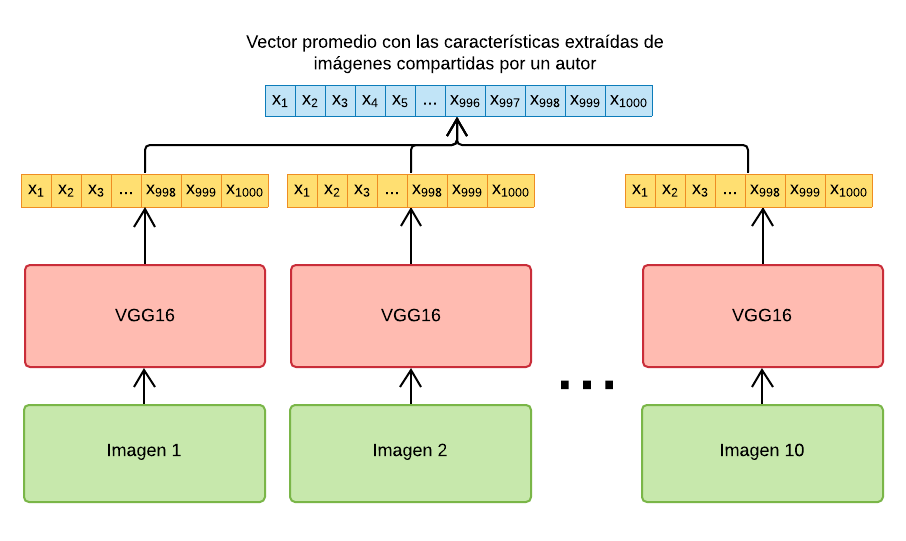
\includegraphics[scale=0.3]{img/features_extraction.png}
    \caption{Esquema de la representación de un autor a través de la extracción
    de características de las 10 imágenes que compartió.}
    \label{fig:img_representation}
\end{figure}

\subsection{Esquema de clasificación}

Se construyeron siete clasificadores para identificación del género de los autores, 
uno por cada subconjunto de las colecciones de imágenes de usuarios en los tres 
diferentes idiomas. Esto es, dado un conjunto $\mathbb{X} = \{\text{Árabe}, 
\text{Español}, \text{Inglés}\}$, donde cada elemento de $\mathbb{X}$ es una colección
de representaciones de las imágenes de 
usuarios del respectivo idioma, el i-ésimo clasificador se entrenó con una colección 
$X_i \subseteq \mathbb{X}$ y $X_i \neq \varnothing$. Para este trabajo,
el algoritmo de aprendizaje utilizado fue una máquina de vectores de soporte (SVM por 
sus siglas en inglés) con un kernel lineal. Después del entrenamiento 
de cada uno de los posibles clasificadores, éstos se evalúan con una colección $Y \in \mathbb{X}$. 
En la Figura \ref{fig:classifier} se muestra un ejemplo.

\begin{figure}[!h]
    \centering
    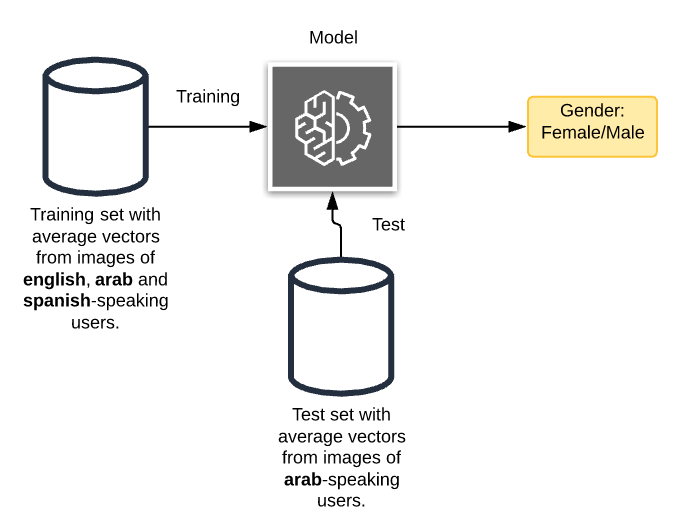
\includegraphics[scale=0.3]{img/classifier_scheme.png}
    \caption{Ejemplo del flujo de entrenamiento y prueba de un modelo entrenado
    con imágenes de usuarios del idioma árabe y español, y evaluado con la colección
    de árabe.}
    \label{fig:classifier}
\end{figure}


\section{Experimentos}

La colección de imágenes utilizada es la ofrecida en la tarea de perfilado de autores del PAN 2018
\cite{rangel_rosso_montes-y-gomez_potthast_stein}, donde se disponen de diez imágenes por cada autor y el número de autores de cada género es el mismo. El Cuadro \ref{table-datasets}
muestra una descripción de los conjuntos de datos utilizados con respecto al número
de usuarios y al idioma de éstos.

La base para comparar el enfoque propuesto son las pruebas monolingües, es decir, aquellos clasificadores entrenados y evaluados con imágenes de usuarios del mismo idioma.
Como los conjuntos de datos están balanceados con respecto al número de mujeres
y de hombres, la medida de evaluación para comparar los distintos clasificadores
es la exactitud, es decir, la proporción de muestras clasificadas correctamente.
% Para la implementación se emplean las bibliotecas de Python para aprendizaje 
% profundo y aprendizaje automático Keras y scikit-learn, respectivamente. La primera
% para extraer las representaciones de las imágenes de los usuarios con el modelo
% pre-entrenado (VGG16) y la segunda para construir y evaluar las SVM
% para identificación de género. 
% Todo el software desarrollado está disponible en
% \url{https://github.com/ivanfeliciano/image-labeling-author-profiling}.

\begin{table}[]
\caption{Número de usuarios por cada idioma para los conjuntos de entrenamiento y de prueba.}\label{table-datasets}
\centering
\begin{tabular}{|l|l|l|l|l|}
\hline
              & Árabe & Español & Inglés & Total \\ \hline
Entrenamiento & 1500  & 3000    & 3000   & 7500  \\ \hline
Prueba        & 1000  & 2200    & 1900   & 5100  \\ \hline
Total         & 2500  & 4900    & 5200   & 12600 \\ \hline
\end{tabular}
\end{table}

\section{Resultados}

En el Cuadro \ref{results_accuracy} se reportan los 
resultados de la evaluación de los diferentes clasificadores
entrenados con imágenes de los subconjuntos de $\mathbb{X}$.
El Cuadro \ref{results_accuracy} muestra un ligero
incremento utilizando las colecciones de los tres idiomas
con respecto a usar la colección de
cada idioma por separado.
El aumento más notable en exactitud corresponde al
conjunto de imágenes de usuarios en árabe. 
% Podemos suponer
% que esto se debe al aumento de vectores en el conjunto de 
% entrenamiento.


\begin{table}[]
\centering
\caption{Exactitud obtenida por las pruebas monolimgües y crosslingües.}
\label{results_accuracy}
\begin{tabular}{|l|l|l|}
\hline
Idioma entrenamiento & Idioma de prueba & Exactitud \\ \hline
Árabe                & Árabe            & 0.68      \\ \hline
Español              & Español          & 0.67      \\ \hline
Inglés               & Inglés           & \textbf{0.70}      \\ \hline
Árabe                & Inglés           & 0.63      \\ \cline{2-3} 
                     & Español          & 0.63      \\ \hline
Español              & Inglés           & 0.67      \\ \cline{2-3} 
                     & Árabe            & 0.70      \\ \hline
Inglés               & Español          & 0.67      \\ \cline{2-3} 
                     & Árabe            & 0.69      \\ \hline
Árabe Español        & Inglés           & 0.68      \\ \cline{2-3} 
                     & Español          & 0.67      \\ \cline{2-3} 
                     & Árabe            & \textbf{0.71}      \\ \hline
Árabe Inglés         & Inglés           & 0.68      \\ \cline{2-3} 
                     & Español          & 0.66      \\ \cline{2-3} 
                     & Árabe            & 0.69      \\ \hline
Español Inglés       & Inglés           & \textbf{0.70}      \\ \cline{2-3} 
                     & Español          & \textbf{0.68}      \\ \cline{2-3} 
                     & Árabe            & 0.70      \\ \hline
Árabe Español Inglés & Inglés           & \textbf{0.70}      \\ \cline{2-3} 
                     & Español          & \textbf{0.68}      \\ \cline{2-3} 
                     & Árabe            & \textbf{0.71}      \\ \hline
\end{tabular}
\end{table}

Como la SVM no ofrece una explicación sobre la clasificación,
realizamos un análisis de los atributos en los vectores que representan 
a los usuarios.
Este análisis se hizo con los atributos 
frecuentes entre los géneros e idiomas y obteniendo aquellos
con mayor ganancia de información.

Para la primera parte se obtuvo un vector para cada género en cada idioma
a partir de las suma de los vectores que representan a cada usuario, agrupados
por género. La Figura \ref{img-vgg16-freqs} muestra nubes de palabras con 
50 de los atributos con la suma más alta.

\begin{figure}[h]
\centering
\subfloat[Género: Femenino. Idioma: Árabe.]{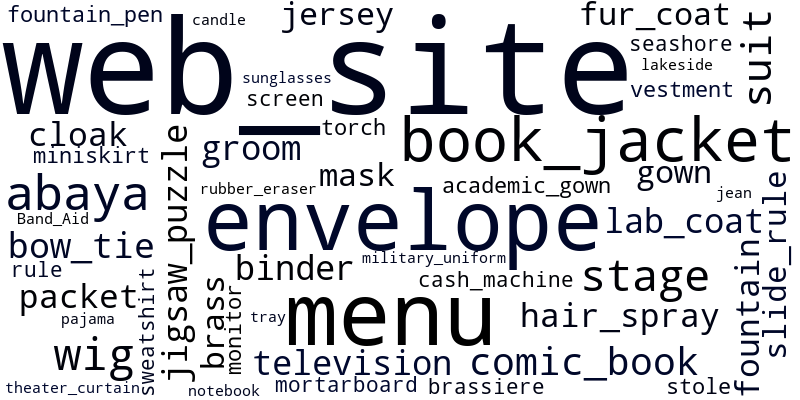
\includegraphics[scale=0.2]{img/AR_F_wordcloud.png}}
\qquad
\subfloat[Género: Masculino. Idioma: Árabe.]{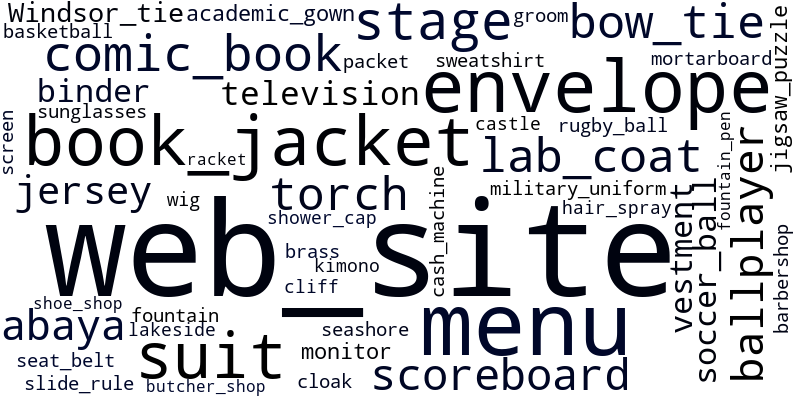
\includegraphics[scale=0.2]{img/AR_M_wordcloud.png}}\\
\subfloat[Género: Femenino. Idioma: Español.]{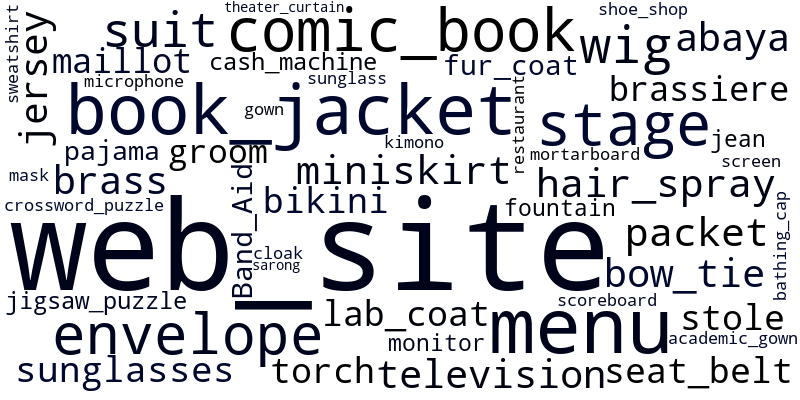
\includegraphics[scale=0.2]{img/ES_F_wordcloud.png}}\qquad
\subfloat[Género: Masculino. Idioma: Español.]{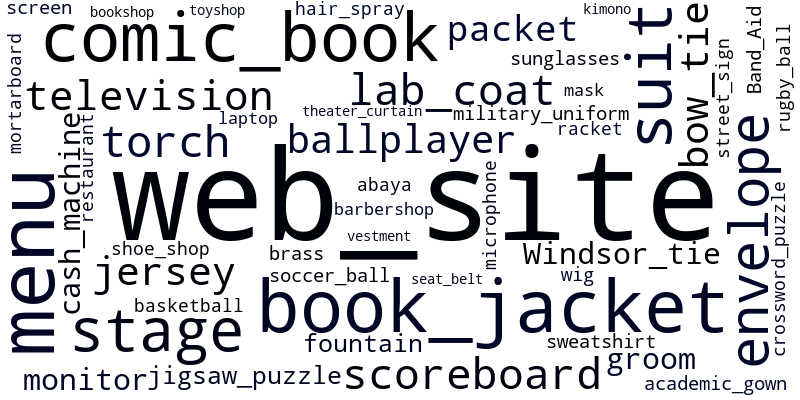
\includegraphics[scale=0.2]{img/ES_M_wordcloud.png}}\\ 
\subfloat[Género: Femenino. Idioma: Inglés.]{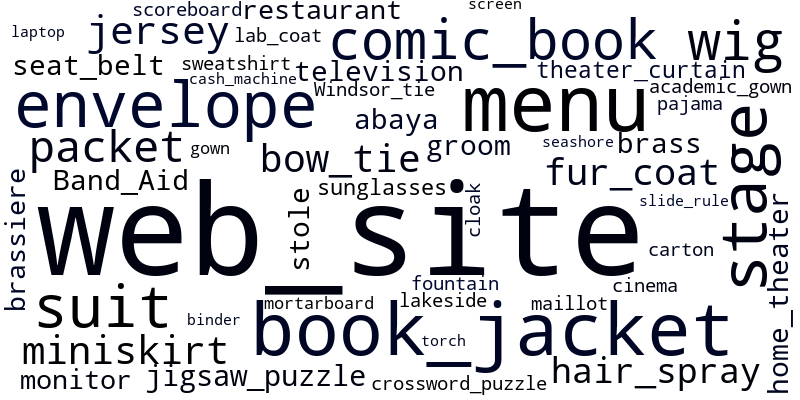
\includegraphics[scale=0.2]{img/EN_F_wordcloud.png}}\qquad
\subfloat[Género: Masculino. Idioma: Inglés.]{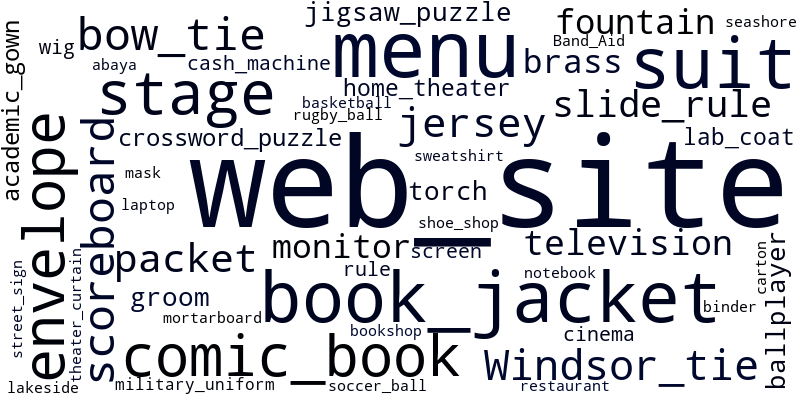
\includegraphics[scale=0.2]{img/EN_M_wordcloud.png}}
\caption{Nubes de palabras de las sumas de vectores de los hombres y mujeres para las características obtenidas con el modelo VGG16. Se muestran los 50 atributos con valores de la suma más altos.}
\label{img-vgg16-freqs}
\end{figure}


De la Figura \ref{img-vgg16-freqs} podemos observar atributos 
con las sumas más altas  que comparten entre géneros e idiomas. Por ejemplo,
algunos de estos atributos son: \texttt{web site}, \texttt{book jacket}, \texttt{envelope}, \texttt{comic book} y \texttt{menu}.

Además, se obtuvo el coeficiente correlación y el índice de Jaccard de los
vectores suma entre todos los pares de idiomas y géneros.
Estos vectores suma sólo contienen los valores para los 100 atributos
con valores más altos. 
Los Cuadros \ref{table:men-vs-men}, \ref{table:women-vs-women}, \ref{table:women-vs-men} muestran los resultados.
En relación a los valores de los coeficientes de correlación, se 
puede ver que los mismos géneros en diferentes idiomas tienen
valores muy altos. Sin embargo, también géneros diferentes en distintos
idiomas tienen una fuerte correlación. Con base en lo anterior, se puede
deducir que existen sólo algunos atributos sobre los que
recae la representación del género de los autores.

Con respecto al índice de Jaccard para medir la similitud entre los conjuntos
de tamaño 100 de atributos entre los diferentes idiomas y géneros se puede 
ver que los pares de conjuntos más similares son entre hombres de los
idiomas: inglés - arabe e inglés - español y entre mujeres de español - inglés. Por el contrario,
los conjuntos menos similares son entre hombres y mujeres de los idiomas:
español - árabe, inglés - árabe y español - inglés.

% {'hair_spray', 'brassiere', 'stole', 'Blenheim_spaniel', 'Persian_cat', 'overskirt', 'miniskirt', 'ballplayer', 'velvet', 'lipstick', 'wig', 'bath_towel', 'Shih-Tzu', 'spatula', 'suit'}


\begin{table}[]
\centering
\caption{Correlación e índice de Jaccard para hombres en los distintos idiomas.}
\label{table:men-vs-men}
\begin{tabular}{|l|l|l|}
\hline
& \begin{tabular}[c]{@{}l@{}}Coeficiente de \\ correlación\end{tabular} & Índice de Jaccard \\ \hline
Árabe-Español              & 0.985                                                                 & 0.681          \\ \hline
Árabe-Inglés               & 0.986                                                                 & 0.724          \\ \hline
Español-Inglés             & 0.996                                                                 & 0.739          \\ \hline
\end{tabular}
\end{table}

\begin{table}[]
\centering
\caption{Correlación e índice de Jaccard para mujeres en los distintos idiomas.}
\label{table:women-vs-women}
\begin{tabular}{|l|l|l|}
\hline
& \begin{tabular}[c]{@{}l@{}}Coeficiente de \\ correlación\end{tabular} & Índice de Jaccard \\ \hline
Árabe-Español   & 0.973                      & 0.667          \\ \hline
Árabe-Inglés    & 0.976                      & 0.653          \\ \hline
Español-Inglés  & 0.997                      & 0.802          \\ \hline
\end{tabular}
\end{table}

\begin{table}[!htb]
    \caption{Correlación (izquierda) e índice de Jaccard (derecha) entre hombres
    y mujeres de los distintos idiomas.}
    \label{table:women-vs-men}
    \begin{minipage}{.5\linewidth}
        \centering
        % \caption{Correlación Hombres-Mujeres}
        \begin{tabular}{|l|l|l|l|}
        \hline
        \diagbox{Hombres}{Mujeres} & Árabe & Español & Inglés \\ \hline
        Árabe   & 0.982 & 0.977   & 0.980  \\ \hline
        Español & 0.962 & 0.990   & 0.990  \\ \hline
        Inglés  & 0.964 & 0.987   & 0.991  \\ \hline
        \end{tabular}
    \end{minipage}%
    \begin{minipage}{.5\linewidth}
        \centering
        % \caption{Jaccard Hombres vs Mujeres}
        
        \begin{tabular}{|l|l|l|l|}
        \hline
         \diagbox{Hombres}{Mujeres}        & Árabe & Español & Inglés \\ \hline
        Árabe   & 0.626 & 0.626   & 0.613  \\ \hline
        Español & 0.563 & 0.681   & 0.667  \\ \hline
        Inglés  & 0.550 & 0.587   & 0.626  \\ \hline
\end{tabular}
    \end{minipage} 
\end{table}
\begin{table}[]

\end{table}

El otro análisis se realizó con una perspectiva 
de selección de atributos, obteniendo la ganancia de información 
de los atributos en cada idioma. En la Figura \ref{img-gi} se muestran
diagramas con los 25 atributos con mayor ganancia de información para cada par de 
idiomas. La intersección de los 25 atributos para los tres conjuntos de idiomas 
son cuatro: \texttt{brassiere}, \texttt{lipstick}, \texttt{velvet} y 
\texttt{bath towel}. A partir de estas cuatro características importantes
se realizó un análisis de fotografías cuyos valores sobre esos atributos
fueron altos. De las Figuras \ref{fig:towel}, \ref{fig:brassiere}, 
\ref{fig:lipstick}, \ref{fig:velvet} se puede ver las imágenes compartidas
y el resultado de los modelos de identificacióń de género, el cual fue el género
femenino utilizando todos lo modelos, excepto en una fotografía en la que dos modelos,
el entrenado con inglés y árabe y el monolingüe inglés, identificaron al autor
como masculino.

Al aumentar la lista a las 100 características con mayor ganancia de información
se consigue una intersección mayor entre los tres idiomas. La intersección
de atributos para 100 características es: \texttt{hair spray}, \texttt{brassiere}, \texttt{stole}, \texttt{Blenheim spaniel}, \texttt{Persian cat}, \texttt{overskirt}, \texttt{miniskirt}, \texttt{ballplayer}, \texttt{velvet}, \texttt{lipstick}, \texttt{wig}, \texttt{bath towel}, \texttt{Shih Tzu}, \texttt{spatula} y \texttt{suit}.

Se realizó el mismo experimento de obtener imágenes que tienen una alta 
probabilidad de contener la característica \texttt{ballplayer}, para
observar a qué género permitía distinguir. En la Figura \ref{fig:ballplayer}
se muestran los resultados para los diferentes idiomas, el género identificado
fue el masculino.


\begin{figure}[h]
\centering
\subfloat{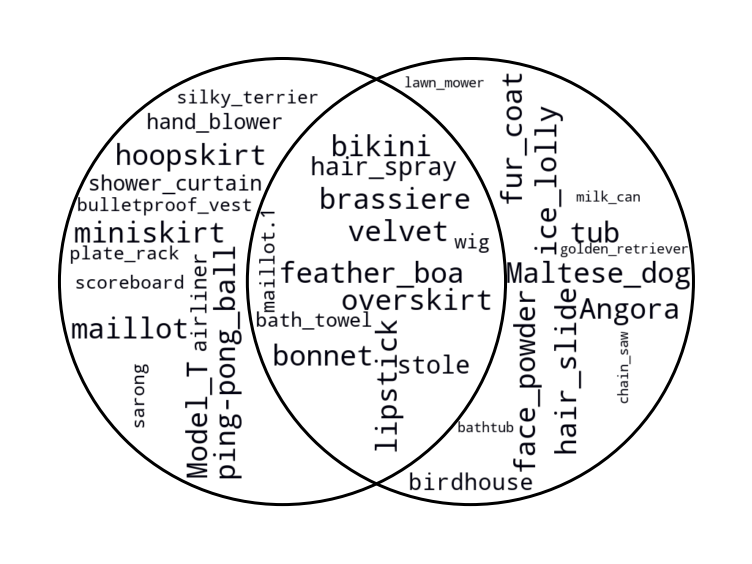
\includegraphics[scale=0.2]{img/en_es_gi.png}}
\subfloat{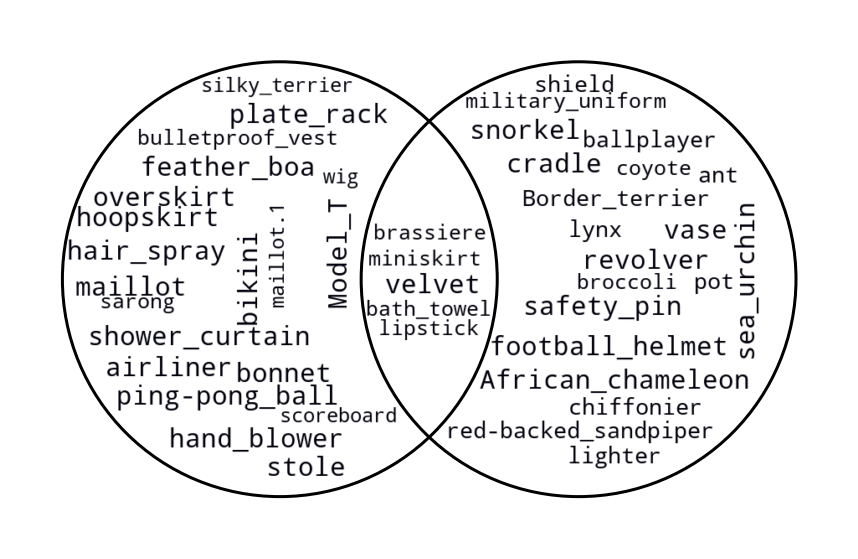
\includegraphics[scale=0.2]{img/en_ar_gi.png}}\\
\subfloat{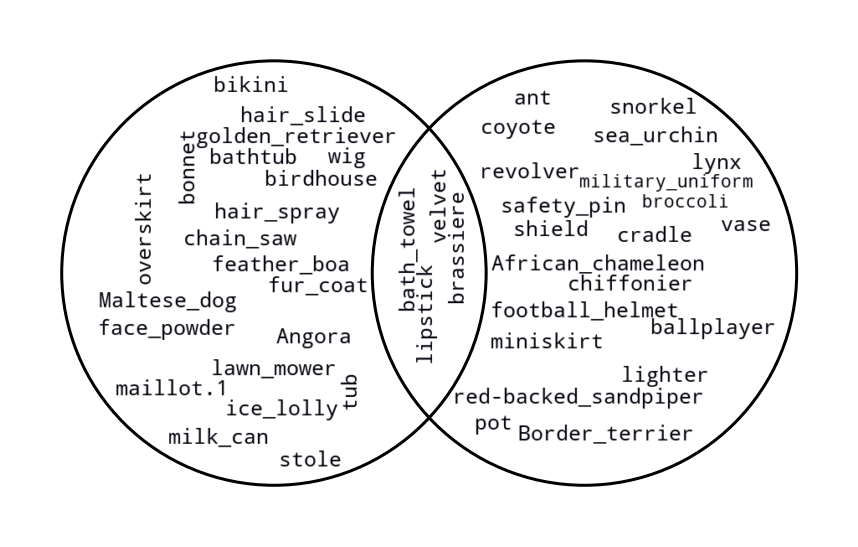
\includegraphics[scale=0.2]{img/es_ar_gi.png}}   
\caption{Intersección de los 25 atributos con mayor ganancia de información.}
\label{img-gi}
\end{figure}



\begin{figure}
    \centering
    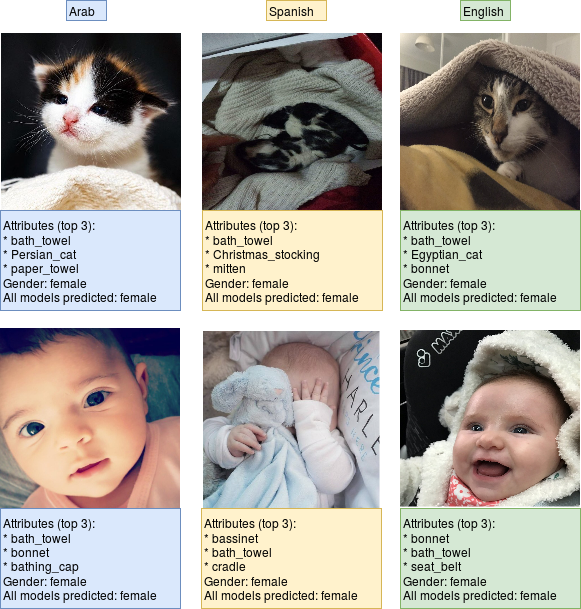
\includegraphics[scale=0.37]{img/best_gi/bath_towel_gi.png}
    \caption{Bath towel}
    \label{fig:towel}
\end{figure}
\begin{figure}
    \centering
    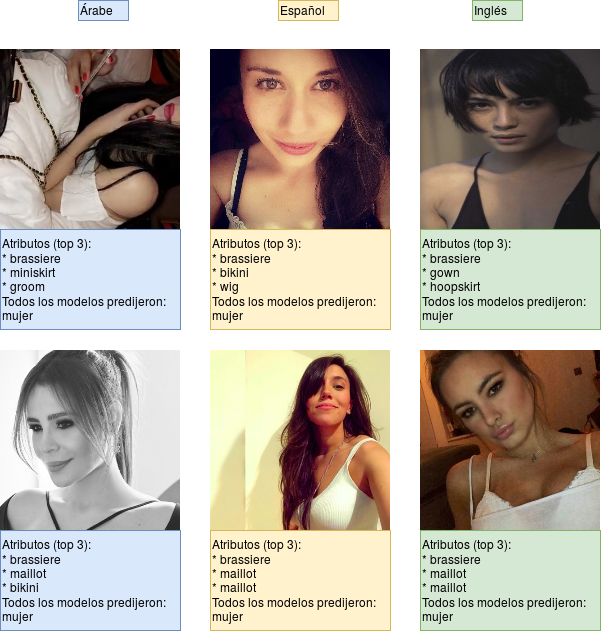
\includegraphics[scale=0.37]{img/best_gi/brassiere_gi.png}
    \caption{Bra}
    \label{fig:brassiere}
\end{figure}
\begin{figure}
    \centering
    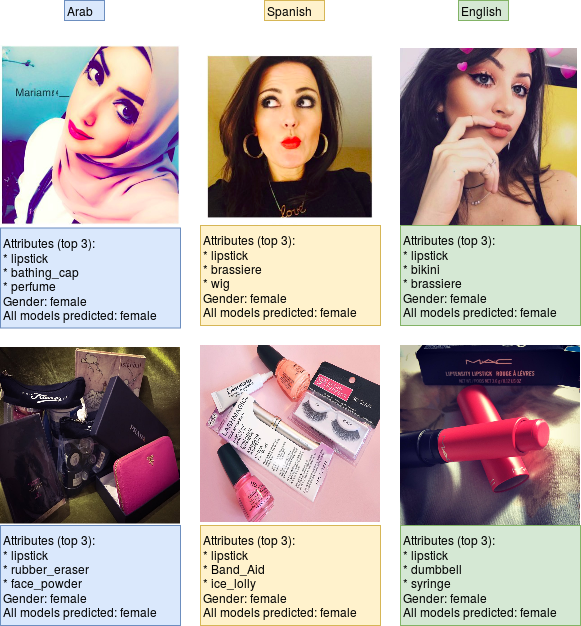
\includegraphics[scale=0.37]{img/best_gi/lipstick_gi.png}
    \caption{Lipstick}
    \label{fig:lipstick}
\end{figure}
\begin{figure}
    \centering
    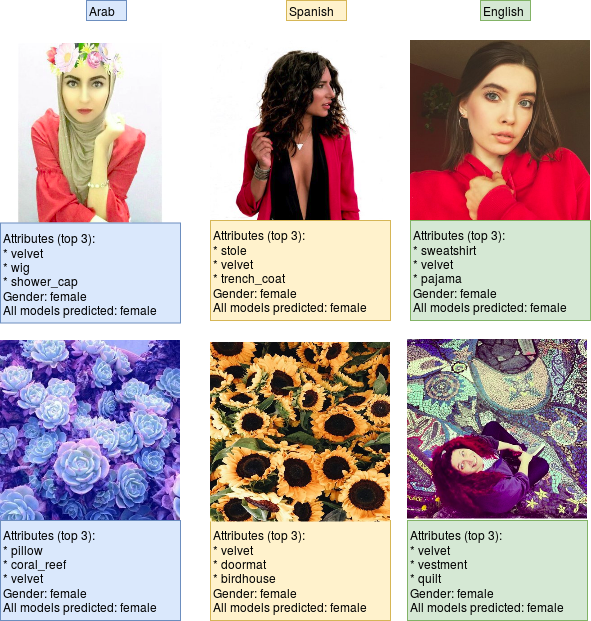
\includegraphics[scale=0.37]{img/best_gi/velvet_gi.png}
    \caption{Velvet}
    \label{fig:velvet}
\end{figure}
\begin{figure}
    \centering
    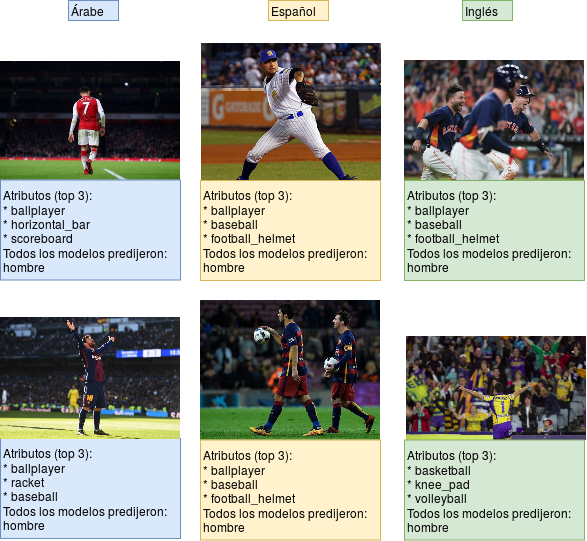
\includegraphics[scale=0.37]{img/best_gi/ball_player_gi.png}
    \caption{Ballplayer}
    \label{fig:ballplayer}
\end{figure}
% \begin{itemize}
%     \item Análisis de resultados.
%     \item Tablas de las combinaciones que se probaron.
%     \item Selección de características.
%     \item Histogramas de ``frecuencias''.
%     \item Correlación entre los vectores de los hombres y mujeres
%     entre los idiomas.
% \end{itemize}

\newpage
\section{Conclusiones y trabajo futuro}
En este trabajo se propuso un esquema crosslingüe para el perfilado de autores
usando las imágenes compartidas por usuarios en tres idiomas. La idea central
es unir las colecciones de varios idiomas para probar si esto mejora el 
desempeño para identificar el género de un usuario de un idioma en específico.
Llevamos a cabo los experimentos utilizando las colecciones de imágenes
provistas en la tarea de perfilado de autores
del PAN 2018. A partir de los resultados obtenidos, se puede ver un 
ligero incremento en la exactitud utilizando todas las colecciones para
entrenar un modelo y probarlo con un idioma por separado.
Además de esto, a través de un análisis de las representaciones
de las imágenes usando atributos semánticos se pudo observar que hay 
atributos importantes para distinguir las clases que coinciden en 
los tres idiomas. Sin embargo, a pesar de que el desempeño obtenido es bueno,
está por debajo del que obtuvieron los autores en \cite{takahashi_tahara_nagatan_miura_taniguchi_ohkuma} que obtuvo
un promedio de 0.7872, el promedio de nuestros mejores clasificadores fue 
de 0.6966. Una posible causa es la limitación de nuestra representación
de cada autor.
\begin{itemize}
    \item ¿El idioma importa? 
    \item ¿Comparten lo mismo los usuarios del género $X$ en el idioma
    $Y$ y los usuarios del género $X$ en el idioma $\hat{Y}$.
    \item ¿Es suficiente el vocabulario con el que cuenta imagenet
    (1000 objetos y escenarios)?
    \item Extender el trabajo usando el enfoque no supervisado.
    \item Vocabulario abierto.
    \item Agrupamiento dentro de cada género.
\end{itemize}

\bibliographystyle{splncs04}
\bibliography{references}

\end{document}
